%%%%%%%%%%%%%%%%%%%%%%%%%%%%%%%%%%%%%%%%%%%%%%%%%%%%%%%%%%%%%%%%%%%%%%%%%%%%%%%%%%%%%%%%%%%%%%%%%%%%%%%%%%%%%%%%%%%%%%%%
\newpage
\chapter {\Large{Handling Libraries}}

An Android library project is a development project that holds shared Android source code and resources. Other Andriod application projects can reference the library project and, at build time, include its compiled sources in their .apk files. Multiple application projects can reference the same library project and any single application project can reference multiple library projects.

\par
Siminov provides mechnism to configure ORM for your library projects. 


\section{Setting up a Library Project}

\begin{enumerate}

	\item \small In the \textbf{Package Explorer}, right-click the library project and select \textbf{Properties}.

	\item \small In the \textbf{Properties} window, select the Andorid properties group at left and locate the \textbf{Library} properties at right.

	\item \small Select the is Library checkbox and click \textbf{Apply}.

	\item \small Click \textbf{OK} to close the properties window.

\end{enumerate}

		\begin{figure}[!htbp]
			\centering
				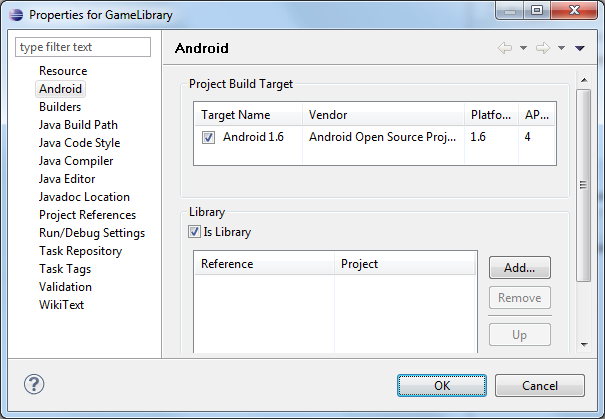
\includegraphics[height=10cm]{Resources/setting_up_a_library_project.png}
		\end{figure}

\newpage
\section{Referencing a library project}
\begin{enumerate}

	\item \small In the \textbf{Package Explorer}, right-click the depedent project and select \textbf{Properties}.

	\item \small In the \textbf{Properties} window, select the Android properties group at left and locate the \textbf{Library} properties at right.
	
	\item \small Click \textbf{Add} to open the \textbf{Project Selection} dialog.

	\item \small From the list of available library project, select a project and click \textbf{OK}.

	\item \small When the dialog closes, click \textbf{Apply} in the \textbf{Properties} window.

	\item \small Click \textbf{OK} to close the \textbf{Properties} window.
	
\end{enumerate}

\newpage
		\begin{figure}[!htbp]
			\centering
				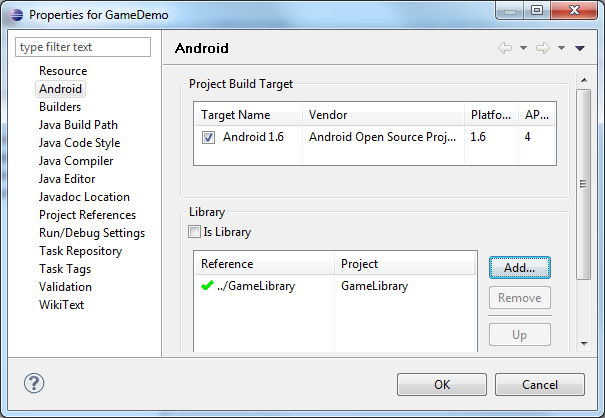
\includegraphics[height=10cm]{Resources/referencing_a_library_project.png}
		\end{figure}

\newpage
\section{Configure Application With Library}

\begin{enumerate}

	\item \small Define LibraryDescriptor.si.xml file for your library project.
	
		\begin{figure}[!htbp]
			\centering
				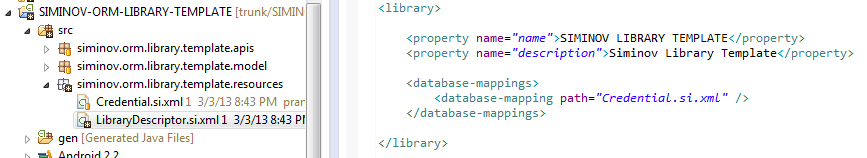
\includegraphics[height=3.5cm]{Resources/siminov_library_template_library_descriptor.png}
		\end{figure}

		\begin{center}
			\colorbox{grey}{
			\parbox[t]{.8\linewidth}{
				\fontsize{11pt}{11pt}\selectfont % The first argument for fontsize is the font size of the text and the second is the line spacing - you may need to play with these for your particular title
				\vspace*{0.1cm} % Space between the start of the title and the top of the grey box
		
				\hfill \textbf{Note} \\
					LibraryDescriptor.si.xml file should not be place in assets folder. Create new package and place all descriptors in that.

				\vspace*{0.0cm} % Space between the end of the title and the bottom of the grey box
				}
			}

		\end{center}


	\item \small Configure LibraryDescriptor.si.xml in your application.
			
		\begin{figure}[!htbp]
			\centering
				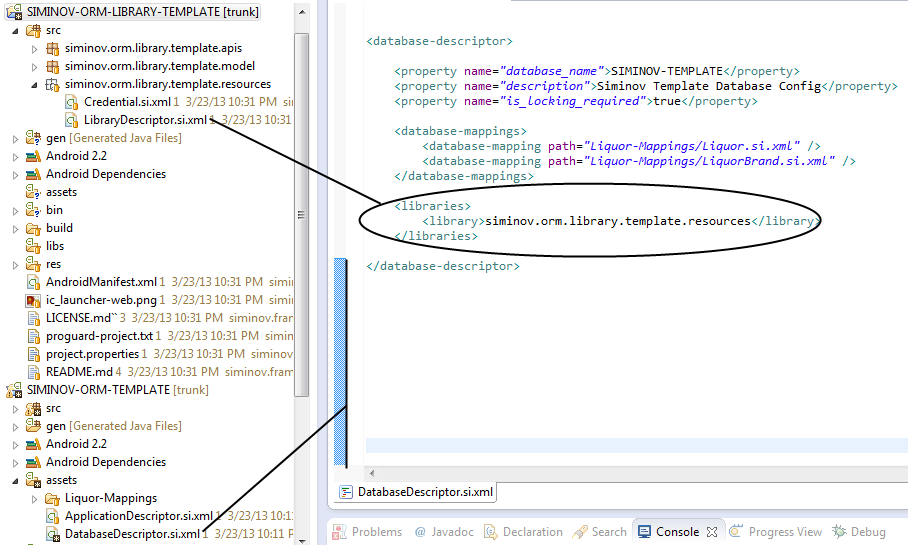
\includegraphics[height=10cm]{Resources/siminov_library_template_configure.png}
		\end{figure}

		\begin{center}
			\colorbox{grey}{
			\parbox[t]{.8\linewidth}{
				\fontsize{11pt}{11pt}\selectfont % The first argument for fontsize is the font size of the text and the second is the line spacing - you may need to play with these for your particular title
				\vspace*{0.1cm} % Space between the start of the title and the top of the grey box
		
				\hfill \textbf{Note} \\
					While configuring DatabaseDescriptor.si.xml file you need to provide full library package name in which LibraryDescriptor.si.xml file is defined.

				\vspace*{0.0cm} % Space between the end of the title and the bottom of the grey box
				}
			}

		\end{center}



\end{enumerate}
